\section{Unix}
\subsection{Historique}
Créé en 1969 par Ken Thompson et Dennis Ritchie suite à l'idéologie qu'un
système d'exploitation performant pour un usage interactif n'avait nul besoin
d'être coûteux, que ce soit en termes d'ordinateur d'accueil ou de développement
humain. Néanmoins, ce n'est qu'en octobre 1973 qu'UNIX prendra sa place au sein
du monde informatique, les codes sources furent disponibles et modifiables par
la communauté qui apporta à UNIX de meilleurs outils. De nos jours, UNIX fait
partie des systèmes d'exploitation les plus répandus bien qu'il ait été conçu
et développé il y a quelques dizaines d'années. \\

Les principales raisons faisant qu'UNIX soit encore utilisé aujourd'hui sont
notamment dues à sa robustesse et à quelques fonctionnalités bien élaborées dès
sa conception. De plus, celui-ci possède l'avantage de n'être lié à aucune
architecture ni aucun constructeur particulier. Il en existe de nombreuses versions,
y compris les \textit{UNIX-like} qui s'autoproclament être un système
d'exploitation parfaitement compatible avec UNIX en n'ayant jamais obtenu la
spécification UNIX. Parmi eux, on y trouve la plupart de systèmes gratuits
et/ou open source dont les plus connus sont GNU/Linux et FreeBSD. \\

Ces versions ont l'avantage de pouvoir exploiter la quasi-totalité du matériel
informatique disponible sur le marché que ce soit sur des serveurs volumineux,
de gros calculateurs ou des ordinateurs domestiques. De même, divers boîtiers
réseau (\textit{routeurs, switches, ...}) fonctionnent sous UNIX et certains
ordinateurs de poche (\textit{PDA}) et smartphones sont équipés d'UNIX. \\

Cependant, avant les années 1990, UNIX n'a été disponible que dans le monde
scientifique avec une interface utilisateur austère. Suite à l'apport du
protocole graphique X-Window développé par le MIT, tout utilisateur peut
utiliser une station UNIX à l'aide d'une souris et d'un écran graphique, même
s'il est recommandé d'apprendre le fonctionnement interne ainsi que des
commandes spécifiques afin d'exploiter au maximum les possibilités d'UNIX,
notamment pour les administrateurs système qui doivent souvent développer des
scripts afin d'automatiser certaines tâches. \\

En 1991, Linus Torvalds - étudiant en informatique à l'Université d'Helsinki -
conçoit le noyau Linux suite à une déception du système d'exploitation MS-DOS
et à cause d'un manque de bonne émulation de terminal proposé par MINIX, un
clone open source d'UNIX développé par Andrew Tanenbaum.

\newpage

\subsection{Composition}
Le système d'exploitation UNIX comporte un ensemble d'outils mis à disposition
de l'utilisateur, et son rôle principal est la répartition automatique des
ressources de manière équitable entre les différentes tâches et utilisateurs. \\
Globalement, UNIX est composé des éléments suivants : \\

\begin{itemize}
\item Un noyau dont le rôle est d'assurer la gestion de la mémoire, les
échanges d'entrées/sorties de bas niveau ainsi que de la répartition des
tâches. \\

\item Un ensemble d'utilitaires de base : \\

  \begin{itemize}
  \item[$\bullet$] Divers interpréteurs de commande qui permettent d'exécuter
des commandes utiles à la manipulation de fichiers, de gestion de processus
(\textit{activité du système}), de communications (\textit{tubes, sockets
TCP/IP intégrés}), ... De plus, ces interpréteurs permettent de démarrer des
activités séparées ou communicantes. \\

  \item[$\bullet$] Des éditeurs de textes (\textit{nano, vim}). \\

  \item[$\bullet$] Des compilateurs ainsi que des éditeurs de liens. Néanmoins,
depuis la fermeture des codes sources, le compilateur C n'est plus inclus dans
aucune distribution UNIX. \\

  \item[$\bullet$] Des outils généraux de développement. \\

  \item[$\bullet$] Des utilitaires résidents (\textit{démons}) chargés de rendre
un certain nombre de services de manière transparente.
  \end{itemize}

  \begin{figure}[!h]
    \centering
    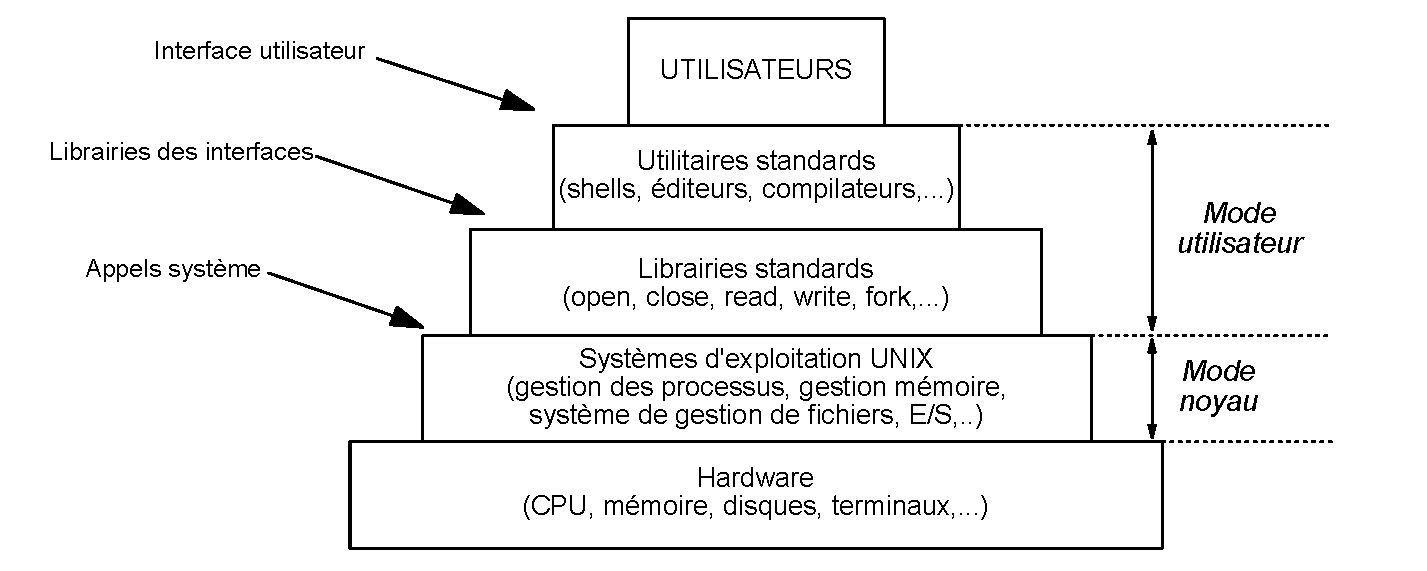
\includegraphics[scale=0.5]
    {textures/images/unix/composition.pdf}
    \caption{Composition d'UNIX}
  \end{figure}
\end{itemize}

\clearpage

\subsection{Distributions}
Elles sont composées d'un ensemble de logiciels définis en fonction de la
distribution choisie et d'un système d'exploitation comportant un noyau. Linux
en possède un très grand nombre en fonction des besoins de l'utilisateur. \\

Exemples de distributions : \\

\begin{itemize}
\item Ubuntu : distribution fournissant un système convivial et ergonomique
pour le grand public. Celui-ci ne nécessite pas de réelles connaissances
approfondies. Elle est recommandée pour un utilisateur désirant apprivoiser les
fonctionnalités de base qu'offre GNU/Linux.

\begin{figure}[!h]
  \center
  
\includegraphics[scale=0.3]
  {textures/images/unix/logos/ubuntu.pdf}
  \caption{Ubuntu}
\end{figure}

\item Red Hat : distribution orientée serveurs et destinée à un public
professionnel. Elle est souvent utilisée par les entreprises.

\begin{figure}[!h]
  \center
  
\includegraphics[scale=0.5]
  {textures/images/unix/logos/redhat.pdf}
  \caption{Red Hat}
\end{figure}

\item Debian : probablement la distribution la plus populaire dont les maîtres
mots sont la stabilité et l'efficacité. Elle concerne un public limité
ayant des notions de base sur GNU/Linux. Seul l'indispensable est
installé par défaut, offrant l'opportunité à l'utilisateur une indépendance par
rapport à sa configuration.

\begin{figure}[!h]
  \center
  
\includegraphics[scale=0.7]
  {textures/images/unix/logos/debian.pdf}
  \caption{Debian}
\end{figure}

\item Fedora : distribution communautaire de Red Hat dont la caractéristique
  première est de suivre les nouveautés technologies. Similaire à Ubuntu, elle
  concerne un grand public et ne nécessite pas de connaissances sur
  GNU/Linux.

\begin{figure}[!h]
  \center
  
\includegraphics[scale=0.5]
  {textures/images/unix/logos/fedora.pdf}
  \caption{Fedora}
\end{figure}

\item Arch Linux : comme Debian, cette distribution - fournissant peu
d'utilitaires d'aide à la configuration - est destinée aux utilisateurs avancés.
Celle-ci sera privilégiée si l'utilisateur veut un système d'exploitation
rapide, léger et flexible. \\

\begin{figure}[!h]
  \center
  
\includegraphics[scale=1.4]
  {textures/images/unix/logos/archlinux.pdf}
  \caption{Arch Linux}
\end{figure}

\item Slackware : c'est la plus vieille des distributions encore utilisées dont l'idéologie est d'être rapide et sans fioritures. Souvent utilisée sur des serveurs, celle-ci n'est maintenue que par très peu de monde dans l'entourage de son
fondateur. \\

\begin{figure}[!h]
  \center
  
\includegraphics[scale=0.5]
  {textures/images/unix/logos/slackware.pdf}
  \caption{Slackware}
\end{figure}

\item (...) \\
\end{itemize}

\newpage

\subsection{Environnements de bureau}
À ne pas confondre avec le système d'exploitation qui s'occupe de gérer les
ressources de l'ordinateur, l'environnement de bureau constitue les
caractéristiques graphiques du système d'exploitation. C'est lui qui permet à
l'utilisateur d'interagir avec son ordinateur. \\

Celui-ci est constitué de divers éléments : \\

\begin{itemize}
\item Bureau : affichage d'un arrière-plan ainsi que d'un ensemble d'icônes. \\

\item Gestionnaire de fenêtres : délimitations des fenêtres par des cadres. \\

\item Barres de menu et des panneaux associés : offre l'accès aux logiciels, à
l'heure, de lister les fenêtres en cours, ... \\

\item Gestionnaire de session : s'occupe des sessions de l'ordinateur. \\

\item Outils graphiques: permettent de contrôler l'ordinateur. \\
\end{itemize}

Divers environnements de bureau : \\

\begin{figure}[!htb]
  \minipage{0.4\textwidth}
  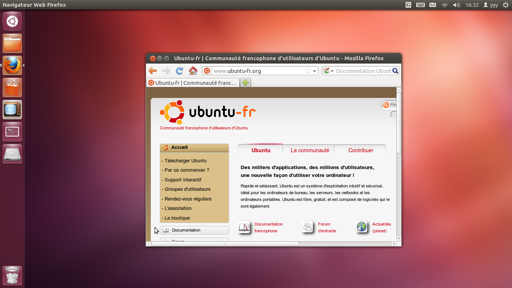
\includegraphics[width=\linewidth]{textures/images/unix/desktop_environment/unity.png}
  \caption{Unity}\label{fig:unity}
  \endminipage\hfill
  \minipage{0.4\textwidth}
  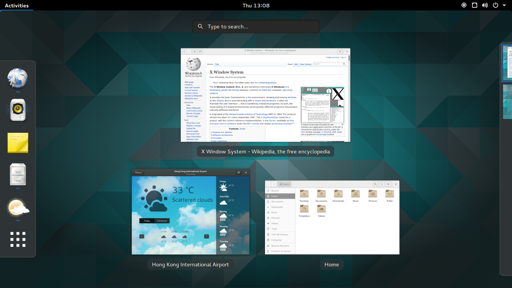
\includegraphics[width=\linewidth]{textures/images/unix/desktop_environment/gnome-shell.png}
  \caption{Gnome Shell}\label{fig:gnome shell}
  \endminipage
\end{figure}

\begin{figure}[!htb]
  \minipage{0.4\textwidth}
  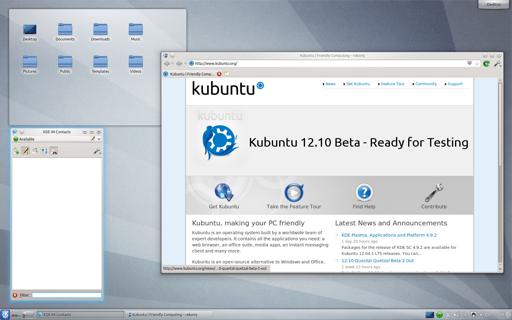
\includegraphics[width=\linewidth]{textures/images/unix/desktop_environment/kde.png}
  \caption{KDE}\label{fig:kde}
  \endminipage\hfill
  \minipage{0.4\textwidth}
  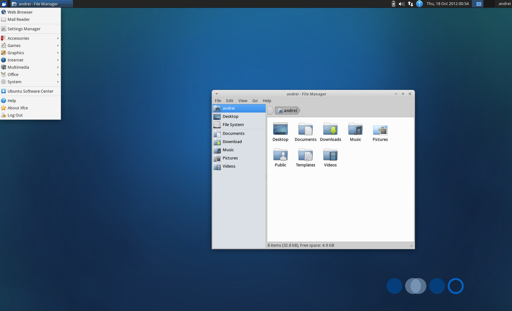
\includegraphics[width=\linewidth]{textures/images/unix/desktop_environment/xfce.png}
  \caption{XFCE}\label{fig:xfce}
  \endminipage
\end{figure}

\newpage

\subsection{Mobilité}
Chez GNU/Linux, il existe un grand nombre de systèmes d’exploitation mobiles et
Android en est le plus connu. Pour tout dire, c'est même le plus utilisé des
systèmes d'exploitation pour smartphones et tablettes avec ses 85 \% de parts de
marché mobile dans le monde. \\

Basé sur un noyau Linux et développé par \textit{Android, Inc.}, il est conçu
pour les smartphones et les tablettes. Trois ans après le rachat de l'entreprise
par Google, le premier smartphone Android - le \textit{T-Mobile G1} - sort aux
États-Unis. Cette première version met en place la \textit{marque de fabrique}
de la plateforme comme les widgets, le Android Market (maintenant nommé
\textit{Play Store}) et l'intégration avancée de Gmail. \\

Le système étant distribué à tout constructeur, Android se trouve être le pendant
de Windows sur mobile: la majorité des mobiles tourne sous une version de Android.
Ce n'est donc pas un hasard si le pourcentage d'utilisation de Windows sur
ordinateurs et quasiment identique à celui de Android. \\

Avec le temps, Android a gagné en fonctionnalités et peut tourner sur encore plus
de dispositifs, comme des télévisions (\textit{Android TV}), des voitures
(\textit{Android Auto}), des smartwatches (\textit{Android Wear}) ainsi que des
ordinateurs (\textit{Android-x86}). \\

Nous en sommes désormais à la sixième version qui se nomme \textit{Marshmallow}.
L'une des particularités est que chaque version possède un nom de sucrerie et
qu'elles se suivent dans l'ordre alphabétique. En voici quelques: \textit{Cupcake},
\textit{Donut}, \textit{Eclair} et \textit{Jelly Bean}, \textit{KitKat}, etc.

  \begin{figure}[!h]
    \centering
    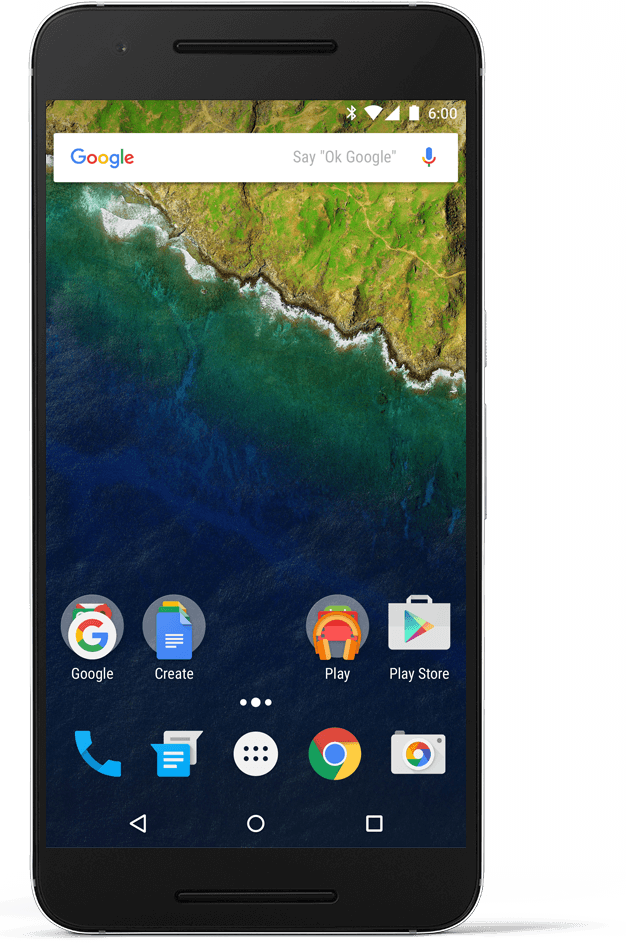
\includegraphics[scale=0.16]
    {textures/images/unix/mobiles/nexus}
    \caption{Nexus 6P sous Android 6.0 Marshmallow}
  \end{figure}

\clearpage
Contrairement aux autres acteurs du marché, GNU/Linux se finance \\
principalement à l'aide de donations, ce qui peut poser divers problèmes pour le
financement de leur développement.  \\

Malgré tout ça, GNU/Linux commence à s'intéresser aux smartphones ainsi qu'aux
tablettes. En effet, Ubuntu Touch est un système d'exploitation développé
pour ces dispositifs. \\

Canonical a d'ailleurs annoncé depuis peu le smartphone « Meizu PRO 5 Ubuntu
Edition » qui est disponible depuis mars 2016.

  \begin{figure}[!h]
    \center
    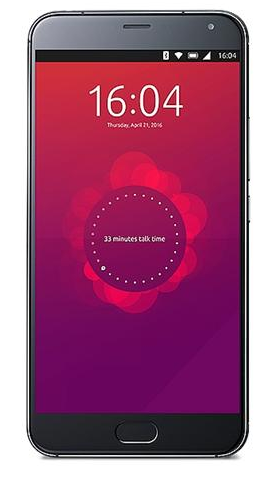
\includegraphics[scale=0.4]
    {textures/images/unix/mobiles/ubuntuTouch}
    \caption{Meizu Pro 5 Ubuntu Edition}
  \end{figure}

Ubuntu Touch à opté pour le glissement de doigt sur l’écran. Un simple
glissement en plein centre de l’écran vers la droite ou la gauche offre la
possibilité de switcher entre les applications principales (\textit{Scopes}).
Et un glissement partant de la bordure de la dalle tactile, ouvre un menu
multitâche similaire à Android. \\

Vu que le système d'exploitation est récent, il est difficile de se prononcer
sur le succès de celui-ci. Cependant, comme Android occupe la majorité du marché
et que celui-ci est composé du noyau Linux, cela sous-entend que cette
technologie pourrait plaire aux utilisateurs d'Android qui désirent d'une
nouvelle interface graphique.
